\documentclass[a4paper,notitlepage,onecolumn]{hitec}  % list options between brackets
\usepackage[pdftex]{graphicx}              % list packages between braces
\usepackage[colorlinks=true,linkcolor=blue]{hyperref}
%\usepackage{bera}% optional: just to have a nice mono-spaced font

%PELARS
%Titles should be done in TRIM SEMIBOLD or FRANKLIN GOTHIC MEDIUM as fallback font. 
%The titles should be done in all caps. 
%The text should be done in Officiana Sans ITC Std or Calibri as fallback font.

%LuaLaTex supporting OpenType fonts
\usepackage{ifluatex}
\ifluatex
\usepackage{fontspec}
\setmainfont{Calibri}
\else
%PDFLaTex we pick a Sans Serif
\usepackage[sfdefault]{cabin}
\usepackage[T1]{fontenc}
%\renewcommand{\familydefault}{\sfdefault}
\fi
\usepackage{listings}
\usepackage{xcolor}
%\usepackage[english]{babel}
%\usepackage[latin1]{inputenc}
\usepackage{longtable}
\usepackage{acro}
\usepackage{multirow}
\usepackage{amsmath}
\usepackage{array}
%\usepackage{natbib}
\usepackage{enumerate}
\usepackage[section]{extraplaceins}
\usepackage{booktabs}
\let\footruleskip\undefined
\usepackage{fancyhdr}
%\usepackage{apacite}
\usepackage[strict]{changepage}
\graphicspath{{./figures/}}

\newcommand{\itemb}[1]{\item \textbf{#1}:}


\colorlet{punct}{red!60!black}
\definecolor{background}{HTML}{EEEEEE}
\definecolor{delim}{RGB}{20,105,176}
\colorlet{numb}{magenta!60!black}
\usepackage{upquote}
\usepackage{color}
\definecolor{editorGray}{rgb}{0.95, 0.95, 0.95}
\definecolor{editorOcher}{rgb}{1, 0.5, 0} % #FF7F00 -> rgb(239, 169, 0)
\definecolor{editorGreen}{rgb}{0, 0.5, 0} % #007C00 -> rgb(0, 124, 0)
\usepackage{upquote}
\usepackage{listings}

\lstset{%
	% General design
	%backgroundcolor=\color{editorGray},
	basicstyle={\normalfont\ttfamily},   
	frame=lines,
	% line-numbers
	xleftmargin={0.75cm},
	%numbers=left,
	stepnumber=1,
	firstnumber=1,
	numberfirstline=true,	
	% Code design
	identifierstyle=\color{black},
	keywordstyle=\color{blue}\bfseries,
	ndkeywordstyle=\color{editorGreen}\bfseries,
	stringstyle=\color{editorOcher}\ttfamily,
	commentstyle=\color{darkgray}\ttfamily,
	tabsize=2,
	showtabs=false,
	showspaces=false,
	showstringspaces=false,
	extendedchars=true,
	breaklines=true
}

\lstdefinelanguage{HTML5}{
	language=html,
	sensitive=true,	
	alsoletter={<>=-},	
	morecomment=[s]{<!-}{-->},
	tag=[s],
	otherkeywords={
		% General
		>,
		% Standard tags
		<!DOCTYPE,
		</html, <html, <head, <title, </title, <style, </style, <link, </head, <meta, />,
		% body
		</body, <body,
		% Divs
		</div, <div, </div>, 
		% Paragraphs
		</p, <p, </p>,
		% scripts
		</script, <script,
		% More tags...
		<canvas, /canvas>, <svg, <rect, <animateTransform, </rect>, </svg>, <video, <source, <iframe, </iframe>, </video>, <image, </image>
	},
	ndkeywords={
		% General
		=,
		% HTML attributes
		charset=, src=, id=, width=, height=, style=, type=, rel=, href=,
		% SVG attributes
		fill=, attributeName=, begin=, dur=, from=, to=, poster=, controls=, x=, y=, repeatCount=, xlink:href=,
		% CSS properties
		margin:, padding:, background-image:, border:, top:, left:, position:, width:, height:,
		% CSS3 properties
		transform:, -moz-transform:, -webkit-transform:,
		animation:, -webkit-animation:,
		transition:,  transition-duration:, transition-property:, transition-timing-function:,
	}
}


\lstdefinelanguage{json}{
	basicstyle=\normalfont\ttfamily,
	%numbers=left,
	%numberstyle=\scriptsize,
	%stepnumber=1,
	%numbersep=8pt,
	showstringspaces=false,
	breaklines=true,
	frame=lines,
	%backgroundcolor=\color{background},
	literate=
	*{0}{{{\color{numb}0}}}{1}
	{1}{{{\color{numb}1}}}{1}
	{2}{{{\color{numb}2}}}{1}
	{3}{{{\color{numb}3}}}{1}
	{4}{{{\color{numb}4}}}{1}
	{5}{{{\color{numb}5}}}{1}
	{6}{{{\color{numb}6}}}{1}
	{7}{{{\color{numb}7}}}{1}
	{8}{{{\color{numb}8}}}{1}
	{9}{{{\color{numb}9}}}{1}
	{:}{{{\color{punct}{:}}}}{1}
	{,}{{{\color{punct}{,}}}}{1}
	{\{}{{{\color{delim}{\{}}}}{1}
	{\}}{{{\color{delim}{\}}}}}{1}
	{[}{{{\color{delim}{[}}}}{1}
	{]}{{{\color{delim}{]}}}}{1}
}

\DeclareAcronym{IDE}{
	short = IDE ,
	long  = Integrated Development Environment,
	class = acro
}
\DeclareAcronym{REST}{
	short = REST ,
	long  = Representational State Transfer,
	class = acro
}
\DeclareAcronym{JSON}{
	short = JSON ,
	long  = JavaScript Object Notation,
	class = acro
}
\DeclareAcronym{ACL}{
	short = ACL ,
	long  = Access Control List,
	class = acro
}

\begin{document}

\title{$\vcenter{\hbox{
\includegraphics{pelarslogo.png}}}$ Learning Analytics Server Interface}   % type title between braces
\author{Emanuele Ruffaldi\\
		Giacomo Dabisias\\
		Lorenzo Landolfi\\PERCRO, Scuola superiore S.Anna}         % type author(s) between braces
\date{31 July 2016}    % type date between braces
\maketitle
\pagestyle{fancy}
\fancyhead[]{}
\fancyfoot[]{}
\fancyfoot[C] {{$\vcenter{\hbox{
\includegraphics{pelarslogo.png}}}$}}
%\fancyhead[CO,CE]{TECHOPT Experiment}
\fancyfoot[RO, LE] {\thepage}

%\begin{abstract}
%\end{abstract}

\tableofcontents 

\printacronyms[include-classes=acro,name=Acronyms]


\section{Introduction}
This document introduces the PELARS server functionalities and the instructions for user access, data management and development.

\section{User registration}
In order to get access to the services available on the server, any user has to be in possession of an active account. It is possible to create a new account by clicking on the subscribe button at \url{http://pelars.sssup.it/pelars/}.\\
You must fill in the form with the requested data and then click the submit button. If the data is correct, a success message will appear and you will be redirected to the login page. The newly created account is in PENDING state and the server administrator will validate the provided information making it ACTIVE. At the moment SSSA administers the server so the account validation time is not immediate
After validation, if you submit the same email and password you submitted in the registration page, you will be granted access to the \ac{REST} operations exposed by the server. 

\section{Server interfaces}
Assuming the user is registered and logged-in there are two ways to interact with the server:
\begin{itemize}
\item Directly with the web-browser
\item Using some script or external program
\end{itemize}

\subsection{Web Browser}
If you want to access the server resources using a web browser, then you have to go to the login page (\url{http://pelars.sssup.it}) and submit your registered data. If the login is successful the server resources will get granted to the web resources by entering the URL. The login is kept across sections thanks to a cookie. \\
First version of entry dashboard is provided at   \ \url{http://pelars.sssup.it/welcome-page.jsp}, allowing you to edit and view the data of your personal sessions, along with some of your personal details.

\subsection{External Program}
If you are developing a program or a servlet that has to interact with the PELARS server the authentication is based on an access token, store it as a variable, and then pass it to any request you are going to perform on your program as a standard {\tt HTTP} parameter named {\tt token}. \\
A very simple example of a javascript/html client can be the one described in the following.\\

\begin{lstlisting}[language=HTML5,firstnumber=1]
<html>
<script type="text/javascript"
src="http://ajax.googleapis.com/ajax/libs/jquery/1.3.2/jquery.min.js"></script>
<script type = "text/javascript" src = "http://pelars.sssup.it/pelars/auth.js"></script>
<script type="text/javascript">
$(document).ready(function() { 
var token = pelars_authenticate();
$.getJSON(
"http://pelars.sssup.it/pelars/session?token="+token,
function(json) {
document.getElementById("id").innerHTML = JSON.stringify(json);
});
});
</script>
<body>
<p id = "id"> </p>
</body>
</html>
\end{lstlisting}

In order to access the resources on the server you have to use the javascript script located at \url{http://pelars.sssup.it/pelars/auth.js}. \\
This file contains the implementation of the function called {\tt pelars\_authenticate}. \\
It asks the user for the PELARS credentials and in case of success, it returns the access token that allow you to access the server resources, else it returns 0. The behaviour of the illustrated html page can be summarized in the following way. \\
As soon as the document is loaded (\$(document).ready), you call the pelars\_authenticate() function and you store the result in the variable token. After this, you perform an automated GET rest request on the {\tt /session} endpoint appending the token as an HTTP parameter. 


\section{Data representation}
Since the messages exchanged with the server are always represented in \ac{JSON}, a standard representation of data which is both machine and human readable,we propose a brief introduction to this kind of representation.\\
A JSON data, or JSON object is always represented in the following way:

\begin{lstlisting}[language=json]
{  
	"field_name_1":"value_1",
	"field_name_2":"value_2",
		...
	"field_name_n":"value_n"
}
\end{lstlisting}
A JSON object is an arbitrary sequence of pairs ({\tt "name" : "value"}) surrounded by curly braces. The name can be any string and the value can be a number, a string, a JSON object, or a JSON array. 
A JSON array is simply a sequence of JSON objects enclosed in brackets. For instance the following is a JSON array.\\
\begin{lstlisting}[language=json] 
[  
	{  
				"field_name_1":"value_1",
      	"field_name_2":"value_2",
					...
      	"field_name_n":"value_n"
   	},
   	{  
      	"field_name_1":"value_1",
      	"field_name_2":"value_2",
					...
      	"field_name_n":"value_n"
   }
]
\end{lstlisting}

\section{Server GET endpoints}
In this section we show how to retrieve data from the server querying its endpoints via REST APIs. In the following paragraphs we assume that words between square brackets are optional parameters of the endpoints, while the ones between curly braces are variables.\\ So for example if an endpoint description contains the following string: {\tt /{foo}/[{bar}]}, then both {\tt foo} and {\tt bar} are variables (i.e. they can be any sequence of letters), but {\tt bar} can be omitted without a parsing error.\\
In case the URL contains {\tt /{foo}/[bar]}, that means that the path parameter located after {\tt foo} must be the exactly string {\tt bar}.

\subsection{Sessions}
You can ask the server for information about PELARS sessions querying the endpoint below. 
\begin{center}
 \url{http://pelars.sssup.it/pelars/session/[{session\_id}]}
\end{center}
If {\tt session\_id} is not specified, you will see the JSON representation of all the sessions you have the permission to see, otherwise, you will see only the representation of the one identified by session\_id.\\
The JSON object representing a session has the following fields: 
\begin{enumerate}
\item\textbf{institution\_address}: the address of the institution in which the session has been opened
\item \textbf{institution\_name}: the name of the institution in which the session has been opened
\item\textbf{session}: a uniquely identifying number for the session
\item \textbf{start}: the date in which the session has started. Such time is expressed in unix epoch milliseconds\footnote{Number of milliseconds that have elapsed since January 1, 1970 (midnight UTC/GMT)}.
\item \textbf{end}: (optional) the date in which the session has been closed, in unix epoch milliseconds
\item \textbf{user}: the registered email of the user who has opened the session
\item \textbf{duration}: (optional) if the session has been closed, it is the number of milliseconds between its opening and closing time
\item \textbf{description}: (optional) a custom description given to the session
\item \textbf{score}: (optional) score assigned to this session (from 1 to 5)
\item \textbf{is\_valid}: boolean stating whether this session is to be considered a valid one or a test one.
\end{enumerate}

The following endpoint can be used to retrieve only the sessions having the {\tt is\_valid} field set to {\tt true}.
\begin{center}
\url{http://pelars.sssup.it/pelars/goodsession}
\end{center}

\paragraph{Examples}
\begin{itemize}
\item \textbf{Request}:  \url{http://pelars.sssup.it/pelars/session/} 
\item \textbf{Response}: 
\begin{lstlisting}[language=json,firstnumber=1]
[  
	...
    {
        "duration": 55667,
        "end": "1454431946402",
        "institution_address": "Malmo",
        "institution_name": "MAH",
        "session": 825,
        "start": "1454431890735",
        "user": "nils.ehrenberg@mah.se"
    },
    {
        "duration": 50082,
        "end": "1454436059292",
        "institution_address": "Malmo",
        "institution_name": "MAH",
        "session": 826,
        "start": "1454436009210",
        "user": "nils.ehrenberg@mah.se"
    },
    {
        "duration": 46545,
        "end": "1454436297001",
        "institution_address": "Malmo",
        "institution_name": "MAH",
        "session": 827,
        "start": "1454436250456",
        "user": "nils.ehrenberg@mah.se"
    },
    {
        "duration": 275267,
        "end": "1454436609812",
        "institution_address": "Malmo",
        "institution_name": "MAH",
        "session": 828,
        "start": "1454436334545",
        "user": "nils.ehrenberg@mah.se"
    },
    ...
]
\end{lstlisting}
As you can see session 188 is still open, while the other ones are not.
\end{itemize}

\begin{itemize}
\item \textbf{Request}:  \url{http://pelars.sssup.it/pelars/session/189} 
\item \textbf{Response}: 
\begin{lstlisting}[language=json,firstnumber=1]
 {  
   	"duration": 1356000,
    "end":"2015/09/03 10:46:51",
    "institution_address":"linz",
    "institution_name":"ars2015",
    "session":189,
    "start":"2015/09/03 10:24:15",
    "user": "table2@ars2015.com"
 }
\end{lstlisting}
\end{itemize}

\subsection{Status}
It is also possible to check whether a session is still online or offline. We refer to an "online session" as a session on which the server is currently receiving data.\\
Via the web-browser such information is accessible through\\ \url{pelars.sssup.it/pelars/status.jsp[?session={session\_id}]}, which is a javascript page with a minimal form user interface. The page is refreshed every three seconds to update the session status information.\\ Alternatively there is also a servlet located at \begin{center} \url{pelars.sssup.it/pelars/live/{session\_id}} 
\end{center}with the same purpose.\\Such servlet supports only the GET method and will answer with one of the following messages.
\begin{lstlisting}[language=json,firstnumber=1]  
{"status":"offline"}
\end{lstlisting}
in case the server is not currently receiving data associated to the queried session.
\begin{lstlisting}[language=json,firstnumber=1]  
{"status":"online"}
\end{lstlisting}
in case data are flowing.

\subsection{Calibration}
The server interface exposes also the following endpoint.
\begin{center}
\url{http://pelars.sssup.it/pelars/calibration/{session\_id}}
\end{center}
The GET performed on such an endpoint returns the entries of the calibration matrix associated to the requested session.\\
We have a calibration matrix for each camera, hence for now one for the kinect and one for the C920.\\
A calibration entity is represented in JSON through the following fields.
\begin{enumerate}
\item\textbf{parameters}: a JSON array of values containing the camera parameters
\item \textbf{session}: PELARS session this calibration belongs to
\item\textbf{type}: the name of the camera the parameters refer to
\end{enumerate}

\paragraph{Example}
\begin{itemize}
\item \textbf{Request}:  \url{http://pelars.sssup.it/pelars/calibration/1098} 
\item \textbf{Response}: 
\begin{lstlisting}[language=json,firstnumber=1]
[
    {
        "parameters": [
            0.05616763234138489,
            -0.9982362389564514,
            -0.01922602951526642,
            0.05583819001913071,
            -0.2063054889440536,
            0.007236991077661514,
            -0.9784608483314514,
            0.3779940009117126,
            0.9768742322921753,
            0.05892426520586014,
            -0.2055351287126541,
            1.283311367034912
        ],
        "session": 1098,
        "type": "webcam"
    },
    {
        "parameters": [
            -0.003767034038901329,
            -0.9997590780258179,
            -0.02162422798573971,
            -0.1105171591043472,
            -0.9058334231376648,
            0.01257205940783024,
            -0.4234475195407867,
            -0.6467799544334412,
            0.4236173629760742,
            0.01799280568957329,
            -0.9056625366210938,
            1.427141666412354
        ],
        "session": 1098,
        "type": "kinect2"
    }
]
\end{lstlisting}
\end{itemize}

\subsection{Multimedia}
The generic multimedia entity description is made by the following fields.

\begin{enumerate}
\item \textbf{data}: the url on which is the actual content of this multimedia is located
\item \textbf{id}: identifier of the multimedia entity
\item \textbf{type}: the type of the multimedia (e.g. text, image, video)
\item \textbf{mimetype}: the mimetype of the multimedia (e.g. plain, png, mp4)
\item \textbf{time}: time at which the multimedia content has been posted to the server. Such time is in unix epoch milliseconds
\item \textbf{session}: identifier of the pelars session this multimedia is associated to
\item \textbf{view}: (optional) present only when the type is "image". Identifies the camera that took the picture and its subject. It can be "workspace" when the picture is taken from the kinect and the subject is the table, "mobile" when it is taken from the mobile tool, "people" when it is taken by the C920 camera, "screen" when it is a screenshot.
\item \textbf{trigger}: (optional) indicates if the content was captured with automatic or manual triggering
\item \textbf{creator}: (optional) indicates the issuer of the creation request
\item \textbf{size}: size in byte of the multimedia content
\end{enumerate}

The URL that follows is used to obtain information about the multimedia sent during a pelars session. 
\begin{center}
\url{http://pelars.sssup.it/pelars/multimedia/{session_id}/[{multimedia_id}]/[{extra}]}
\end{center}
If {\tt multimedia\_id} is not specified we get the representation of all the multimedia posted during the session identified by {\tt session\_id}, else we get the actual content or JSON representation of the multimedia identified by {\tt multimedia\_id}, which can be video, image or text.\\
In case the path parameter {\tt extra} is equal to {\tt thumb}, a thumbnail of the image is returned instead of the whole one.\\
Else, if {\tt extra} is equal to {\tt meta}, then the JSON representation if the entity is returned.
\begin{center}
\url{http://pelars.sssup.it/pelars/multimedia/{session_id}/[{x}]}
\end{center}
The url above instead is used to retrieve all the multimedia content descriptors having type specified by the parameter. \{x\} can be for instance "image" or "text".\\
\{x\} can also be intended as "view" field of a multimedia object.

\paragraph{Examples}
\begin{itemize}
\item \textbf{Request}:  \url{http://pelars.sssup.it/pelars/multimedia/1051} 
\item \textbf{Response}: 
\begin{lstlisting}[language=json,firstnumber=1]
[
{
        "creator": "observer",
        "data": "http://pelars.sssup.it/pelars/multimedia/1609/18186",
        "id": 18186,
        "mimetype": "plain",
        "session": 1609,
        "size": 23,
        "time": 1.467887462363E12,
        "type": "text",
        "view": "mobile"
    },
    {
        "creator": "client",
        "data": "http://pelars.sssup.it/pelars/multimedia/1609/18187",
        "id": 18187,
        "mimetype": "jpg",
        "session": 1609,
        "size": 91839,
        "time": 1.467887467362E12,
        "trigger": "automatic",
        "type": "image",
        "view": "people"
    },
    {
        "creator": "client",
        "data": "http://pelars.sssup.it/pelars/multimedia/1609/18188",
        "id": 18188,
        "mimetype": "png",
        "session": 1609,
        "size": 181324,
        "time": 1.467887467804E12,
        "trigger": "automatic",
        "type": "image",
        "view": "screen"
    },
    {
        "creator": "client",
        "data": "http://pelars.sssup.it/pelars/multimedia/1609/18189",
        "id": 18189,
        "mimetype": "jpg",
        "session": 1609,
        "size": 631374,
        "time": 1.467887468803E12,
        "trigger": "automatic",
        "type": "image",
        "view": "workspace"
    },
 ...
]
\end{lstlisting}
\end{itemize}

\begin{itemize}
\item \textbf{Request}:  \url{http://pelars.sssup.it/pelars/multimedia/542/604} 
\item \textbf{Response}: 
\begin{center}
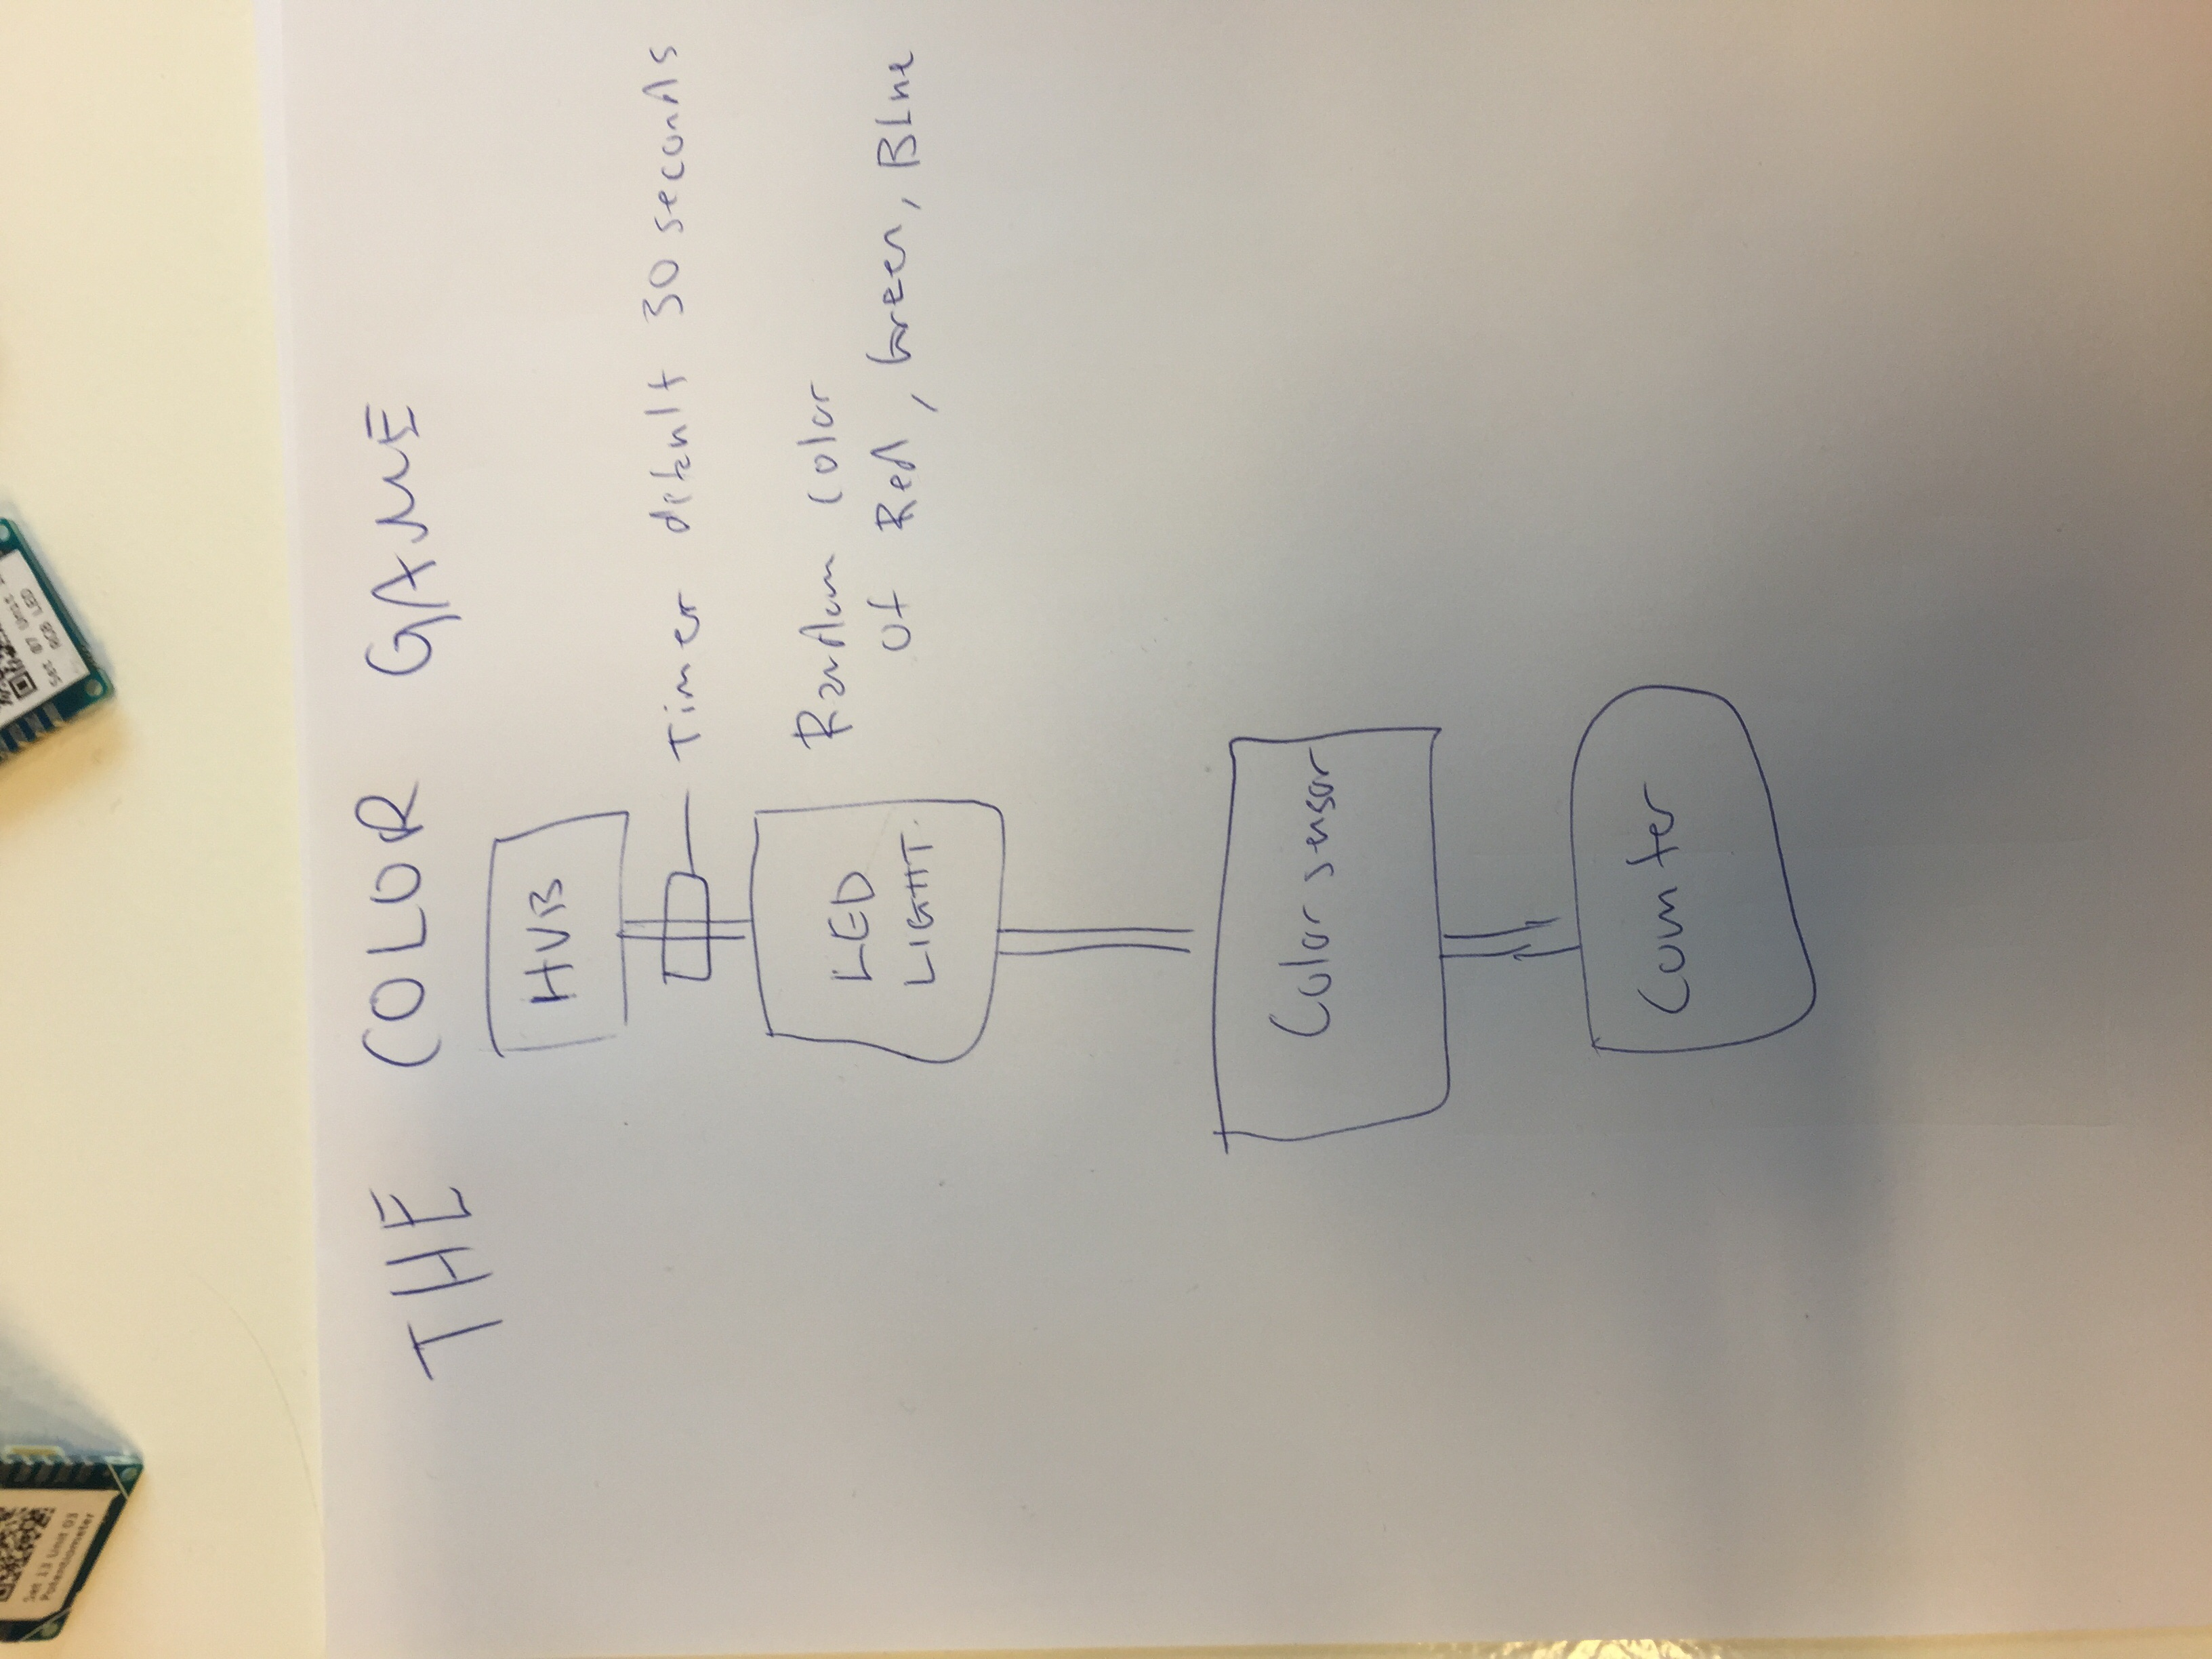
\includegraphics[scale=0.09, angle=-90]{604.jpg}
\end{center}
\end{itemize}

\begin{itemize}
\item \textbf{Request}:  \url{http://pelars.sssup.it/pelars/multimedia/1051/2368/meta}
\item \textbf{Response}: 
\begin{lstlisting}[language=json,firstnumber=1]
{
	"view":"people",
	"size":140540,
	"data":"http://pelars.sssup.it/pelars/multimedia/1051/2368",
	"session":1051,
	"mimetype":"jpg",
	"id":2368,
	"time":1.455638159994E12,
	"type":"image"
}
\end{lstlisting} 
\end{itemize}


\subsection{Data}\label{Data}
In order to get information about the non multimedia data stored by the server you have to perform an HTTP GET on the following URL.
\begin{center}
\url{http://pelars.sssup.it/pelars/data/{session_id}/[{type}?from={value1}&to={value2}&epoch={value3}&phase={value4}]}
\end{center}
This endpoint returns all data samples captured by the collector during the session identified by {\tt session\_id}. 
It is also possible to get only the samples gathered within a certain time interval $[x,y]$ setting two HTTP parameter named "{\tt from}" and "{\tt to}".\\
These two parameters can be specified also after the first call to the endpoint.\\
By default, the extrema of the interval $[x,y]$ are interpreted as milliseconds since the beginning of the session. In case the value of the parameter called "{\tt epoch}" is equal to {\tt true}, then such extrema are interpreted as standard unix epoch milliseconds. 
Moreover it is possible to make sure that the GET on this endpoint returns only the data samples captured during a specific phase.\\
The path parameter {\tt type} allows to return only data of a given type. {\tt type} must be one of the following: "{\tt Face, Hand, Object, Ide, Audio, Particle, Button}", otherwise an error message is returned. Types are described from Section \ref{face} on.\\
All the JSON object returned by this endpoint have some common fields and some unique ones determined by the "{\tt type}" field of the sampled data.\\
The common fields are described below.
\begin{enumerate}
\item\textbf{data\_id}: unique identifier of each data sample
\item\textbf{num}: identifier of the data within a sample interval. Notice that we can have several samples of the same data having the same time (e.g of the same face)
\item \textbf{session}: identifier of the session during which this sample has been taken
\item\textbf{time}: time in which this sample has been taken, in Unix epoch milliseconds.
\item\textbf{type}: type of the data sample
\end{enumerate}

In the following paragraphs we are going to describe the fields of the various data types available from this endpoint.

\subsubsection{Face}
We represent a Face as the three points determining the plane tangent to the surface of the face.\\These points are represented as 3D coordinates in meters, having the origin of the axis fixed to a certain point on the table. In the following we illustrate the name of the fields of the JSON object representing a face.

\begin{enumerate}
\item\textbf{pos\_x0}: abscissa of the leftmost higher point of the rectangle approximating the face
\item\textbf{pos\_x1}: abscissa of the rightmost higher point of the rectangle approximating the face
\item\textbf{pos\_x2}: abscissa of the rightmost lower point of the rectangle approximating the face
\item\textbf{pos\_y0}: ordinate of the leftmost higher point of the rectangle approximating the face
\item\textbf{pos\_y1}: ordinate of the rightmost higher point of the rectangle approximating the face
\item\textbf{pos\_y2}: ordinate of the rightmost lower point of the rectangle approximating the face
\item\textbf{pos\_z0}: height of the leftmost higher point of the rectangle approximating the face
\item\textbf{pos\_z1}: height of the rightmost higher point of the rectangle approximating the face
\item\textbf{pos\_z2}: height of the rightmost lower point of the rectangle approximating the face
\item\textbf{distance}: the approximated distance from camera in meters. 
\end{enumerate}

\subsubsection{Hand}
Hands are identified by the collector thanks to some square markers put on the wrist of the users. Each marker has a unique predefined {\tt id} and we get the position of an hand looking for the center of such markers. \\
We get the 3D coordinates of such markers setting the origin of the axes in a point located on the table. This point is actually identified by a special marker with {\tt id} equal to zero.\\  
\\Hence the characteristics of an hand sample are described by the following list:
\begin{enumerate}
\item\textbf{t\_x, t\_y, t\_z}: translation vector components
\item\textbf{r\_x, r\_y, r\_z, r\_w}: rotation quaternion components
\end{enumerate}

\subsubsection{Audio}
Audio data type represents whether or not there is noise at a certain time during the session, hence the only meaningful feature is the following.
\begin{enumerate}
\item\textbf{value}: number representing the power of the audio signal
\end{enumerate}

\subsubsection{Particle}
This identifies data acquired using the particle.io sensors; it is identified by the sensor name and a generic message sent by the sensor.

\subsection{Button}
This is used to represent button presses. The structure is equal to the one of particle and the "name" field can be "b2" in case the pressed button is the "success button", "b1" in case it is the "frustration button".

\subsubsection{IDE}
This kind of data type represents the feedbacks on the actions performed by the Arduino \ac{IDE}.For the meaning of the following fields contact the Arduino IDE developers.

\begin{enumerate}
\item\textbf{opt}
\item\textbf{action\_id}
\end{enumerate}

\paragraph{Examples}
\begin{itemize}
\item \textbf{Request}:  \url{http://pelars.sssup.it/pelars/data/679} 
\item \textbf{Response}: 
\begin{lstlisting}[language=json,firstnumber=1]
[  
	{  
			"data_id":79222,
			"session":679,
			"time":1.445941731347E12,
			"type":"audio",
			"value":45.87900161743164
   	},
	{  
			"data_id":79223,
			"session":679,
			"time":1.445941731347E12,
			"type":"audio",
			"value":41.15903161545161
	},
	{
        "data_id": 193854,
        "distance": 0.8585148453712463,
        "num": 0,
        "pos_x0": -0.140203,
        "pos_x1": -0.285909,
        "pos_x2": -0.223229,
        "pos_y0": -0.179243,
        "pos_y1": -0.31266,
        "pos_y2": -0.344565,
        "pos_z0": 0.370185,
        "pos_z1": 0.198401,
        "pos_z2": 0.369773,
        "session": 679,
        "time": 1.455546323614E12,
        "type": "face"
    },
    {
        "data_id": 193855,
        "distance": 0.778795599937439,
        "num": 0,
        "pos_x0": -0.204744,
        "pos_x1": -0.35045,
        "pos_x2": -0.28777,
        "pos_y0": -0.142249,
        "pos_y1": -0.275667,
        "pos_y2": -0.307572,
        "pos_z0": 0.399173,
        "pos_z1": 0.227389,
        "pos_z2": 0.398761,
        "session": 679,
        "time": 1.455546324632E12,
        "type": "face"
    },
    {
        "data_id": 193856,
        "distance": 0.7900825142860413,
        "num": 0,
        "pos_x0": -0.194039,
        "pos_x1": -0.339745,
        "pos_x2": -0.277066,
        "pos_y0": -0.146202,
        "pos_y1": -0.279619,
        "pos_y2": -0.311524,
        "pos_z0": 0.397079,
        "pos_z1": 0.225295,
        "pos_z2": 0.396667,
        "session": 679,
        "time": 1.455546325643E12,
        "type": "face"
    },
	{
			"data_id": 53266,
			"num": 784,
			"rw": 0.999999,
			"rx": 3.03634E-4,
			"ry": -0.00108022,
			"rz": -6.08182E-5,
			"session": 679,
			"time": 1.445941737448E12,
			"tx": 1.70484E-4,
			"ty": 1.85072E-4,
			"type": "hand",
			"tz": 6.57141E-8
	},
	{
			"data_id": 53267,
			"num": 960,
			"rw": 0.999381,
			"rx": 3.03188E-4,
			"ry": 6.66941E-4,
			"rz": 0.0351745,
			"session": 679,
			"time": 1.445941737448E12,
			"tx": 0.279248,
			"ty": -0.115026,
			"type": "hand",
			"tz": 6.05506E-6
	}
]
\end{lstlisting}
\end{itemize}

\begin{itemize}
\item\textbf{Request}: \\ \url{http://pelars.sssup.it/pelars/data/679?from=2253&to=9000} 
\item \textbf{Response}: 
\begin{lstlisting}[language=json,firstnumber=1]
[  
   	{  
      	"data_id":79222,
      	"session":679,
      	"time":1.445941739478E12,
      	"type":"audio",
      	"value":45.87900161743164
   	},
   	{
        "data_id": 193854,
        "distance": 0.8585148453712463,
        "num": 0,
        "pos_x0": -0.140203,
        "pos_x1": -0.285909,
        "pos_x2": -0.223229,
        "pos_y0": -0.179243,
        "pos_y1": -0.31266,
        "pos_y2": -0.344565,
        "pos_z0": 0.370185,
        "pos_z1": 0.198401,
        "pos_z2": 0.369773,
        "session": 679,
        "time": 1.445941739478E12,
        "type": "face"
    },
    {
        "data_id": 193855,
        "distance": 0.778795599937439,
        "num": 0,
        "pos_x0": -0.204744,
        "pos_x1": -0.35045,
        "pos_x2": -0.28777,
        "pos_y0": -0.142249,
        "pos_y1": -0.275667,
        "pos_y2": -0.307572,
        "pos_z0": 0.399173,
        "pos_z1": 0.227389,
        "pos_z2": 0.398761,
        "session": 679,
        "time": 1.445941739478E12,
        "type": "face"
    },
]
\end{lstlisting}
\end{itemize}

\subsection{PhaseEntity}\label{PhaseEntity}
It is possible to see how a specific session is divided in phases querying the following URL.
\begin{center}
 \url{http://pelars.sssup.it/pelars/phase/{session\_id}[?from=value1&to=value2&epoch=value3]}
\end{center}
If the {\tt epoch} parameter is not specified or it is set equal to {\tt false}, {\tt from} and {\tt to} are intended as number of seconds elapsed since the beginning of the session. Else they are intended as standard unix epoch time milliseconds. 
Filtering of the response is similar to the one described in \ref{Data}. The values of {\tt from} and {\tt to} are compared with the start time of each phase.\\
The meaning o the fields of the JSON objects returned by the response of an HTTP GET performed on the endpoint above are the following. 
\begin{enumerate}
\item\textbf{data\_id}: unique identifier of the phase
\item\textbf{start}: start time of the phase in unix epoch milliseconds
\item \textbf{end}: end time of the phase in unix epoch milliseconds
\item\textbf{session}: identifier of the session this phase is associated to
\item \textbf{phase}: name the submitter has given to this phase
\end{enumerate}
The time at which a PhaseEntity with name {\tt "phase1"} is posted during a session is the beginning of that phase. 
If $m_1$, $m_2$ and $m_3$ are three phase entities posted one after the other at time respectively $t_1,\ t_2,\ t_3$ such that $m_1$ and $m_2$ are associated to the same phase $p_1$, while $m_3$ is associated with phase $p_2$, then the duration of $p_1$ is considered to be $[t_1,t_3]$.\\ In general a single phase is not associated with a single time interval but with several not overlapping ones, not necessarily consecutive. 

\paragraph{Example}
\begin{itemize}
\item \textbf{Request}:  \url{http://pelars.sssup.it/pelars/phase/678} 
\item \textbf{Response}: 
\begin{lstlisting}[language=json,firstnumber=1]
[
  {
    "data_id": 563,
    "end": 1452788109587,
    "phase": "setup",
    "session": 678,
    "start": 1452788102656
  },
  {
    "data_id": 564,
    "end": 1452788120611,
    "phase": "phase1",
    "session": 678,
    "start": 1452788109587
  },
  {
    "data_id": 565,
    "end": 1452788129060,
    "phase": "phase2",
    "session": 678,
    "start": 1452788120611
  },
  {
    "data_id": 566,
    "end": 1452788132922,
    "phase": "phase3",
    "session": 678,
    "start": 1452788129060
  }
]
\end{lstlisting}
As you can see session 188 is still open, while the other ones are not.
\end{itemize}

\section{Human readable data}
It is also possible to get responses from the endpoints described in the previous section as HTML tables instead that in JSON fromat. This representation can be obtained performing a GET with a browser on the following url: \url{http://pelars.sssup.it/pelars/view.html#[endpoint_path]}.\\
The {\tt endpoint\_path} parameter is actually the name of the endpoint according to the server container (what follows \url{/pelars} in the endpoint described until now).
So for instance to retrieve all the data relative to session 300 during phase "reflect" (equivalent to \url{http://pelars.sssup.it/pelars/data/300?phase=reflect}) it is possible to digit in the browser address bar \\ \url{http://pelars.sssup.it/pelars/view.html#data/300?phase=reflect}
.\\Another example is reported in the following.

\paragraph{Example}
\begin{itemize}
\item\textbf{Request:} \\
\url{http://pelars.sssup.it/pelars/view.html#/multimedia/534}

\item\textbf{Response:}
\begin{center}
\hspace*{-3.3cm}
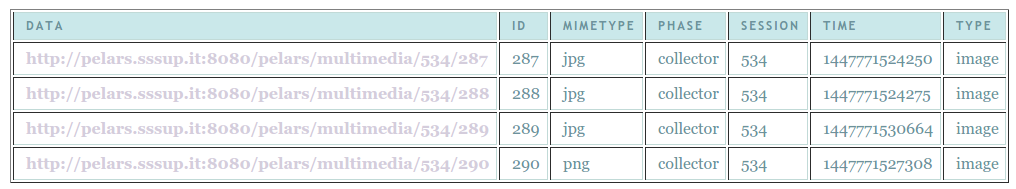
\includegraphics[scale=0.47]{multimedias.png}
\end{center}
\end{itemize}
Moreover we developed a way to visualise the data acquired during a PELARS session in a time-line fashion. \\It is possible to use the Web browser to access the page at address \url{http://pelars.sssup.it/pelars/visualization.jsp[?session=session\_id]}, where a form asks you to type the identifier of a PELARS session. After the submission the page will show a graphical representation of the data gathered during the submitted session lifetime. Figure \ref{fig:fullsession} shows an example of a time-line obtained in such a way.

\begin{figure*}[h]
\hspace*{-3.3cm}
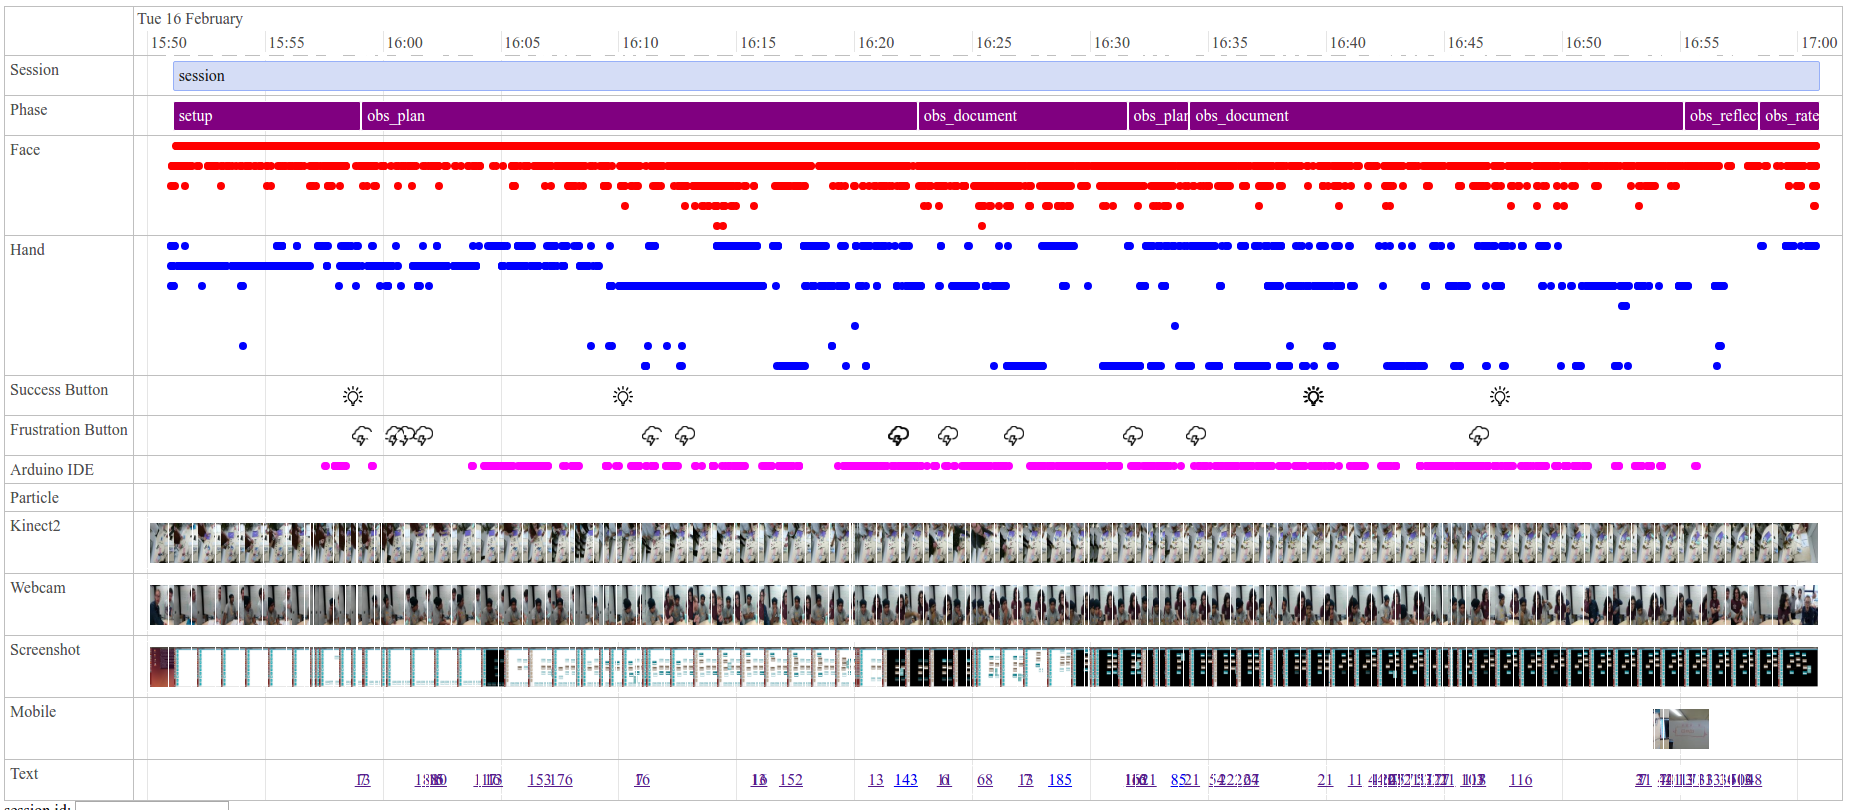
\includegraphics[width=18.5cm, height=8.5cm]{fullsession.png}
\caption{The figure shows the sampled data on a timeline, gathered during a test session, grouped by item type. The top filled bar corresponds to the overall session, below that the phase decomposition is reported. Faces presence is almost continuous. Hand identification is presented with some dots, with one row for every distinct hand; the success and frustration button rows corresponds to button presses. The ide part deals with the Arduino IDE information. It is also possible to see the thumbnails of the submitted images, divided by their point of view}
\label{fig:fullsession}
\end{figure*}

A brief enumeration of the visualization pages and tools provided by the server are reported below.
\begin{itemize}
\item\textbf{Piechart} : this represents a piechart where each "slice" shows the duration of a phase. By hovering above the phase with the mouse you will see the phase name. The bars represent multimedia content and are clickable, redirecting to the content. \url{http://pelars.sssup.it/pelars/piechart.html?session={id}}
\item\textbf{3D Viewer} : this represents the face,hand and camera position in a unique 3D space. It shows the posistion of all components over time calibrated at the beginning of the pelars setup. \url{http://pelars.sssup.it/pelars/3d_viewer.html?session={id}}
\item\textbf{Data card} : this represents a data card with different learing analytics like hand activity and ARduino component connections. \url{http://pelars.sssup.it/pelars/wholeCard.html?session={id}}
\item\textbf{Timeline} : this represents all the pelar session data on a timeline which is draggable and cliccable. \url{http://pelars.sssup.it/pelars/timeline.html?session={id}}
\item\textbf{Audio}: this is the plot of the intensity of all the audio samples recorded during a session. It is also possible to plot a constant threshold by specifying it as an html parameter. \url{http://pelars.sssup.it/pelars/audio.html?session={id}&thresh={th}}
\item\textbf{IDE activity}: this plots the number of IDE samples recorded in intervals of 60 seconds. \url{http://pelars.sssup.it/pelars/program.html?session={id}}
\end{itemize}

\section{ACL}
\ac{ACL} is the policy specifying which users are allowed to perform specific operation and on what objects.\\
In our case the amount of operations allowed to a user are determined by his/her role. The operations are actually the standard basic HTTP methods (GET,PUT,POST,DELETE) and the objects are all the endpoints exposed by the server.\\
For now we have the following roles: 
\begin{itemize}
\item Administrator
\item Researcher
\item viewer
\item Student
\end{itemize}
Currently an administrator can perform any kind of operation on any object. \\A researcher can read (GET) and modify any data associated to a session started by any user sharing the same namespace field (which will be named "research group"). He is also allowed to read and update the information relative to himself (but not his identifier).\\
A viewer has READ rights on all the data but no WRITE rights.\\
A student can only read information about himself.\\
Our \ac{ACL} mechanism allows also to add user's specific rules, where the user's permissions are decided by his/her identifier rather than from his/her role.\\
Such rules override the ones specific to the user's role and they can be either more restrictive or more permissive. Only administrator can grant such rules to other users.\\
For example, if a researcher wants to read  also the data relative to any session of the PELARS database, he can ask such a right to an administrator and the administrator can provide it specifically for him.

\section{Operations}
Some operation have been implemented to extract new data from the stored sessions.\\
Two endpoints are dedicated to this task in the server:
\begin{center}
\url{http://pelars.sssup.it/pelars/op/[op\_id]}  \url{http://pelars.sssup.it/pelars/op/{op\_id}/result}
\end{center}

The first one is intended for submitting operation requests to the server while the second one to get results.
Operations are performed asynchronously: you submit an operation and then poll the server for the result instead of waiting for it. Further operations are to be discussed with the other PELARS partners.\\
Once a request is received by the server,  a message is immediately returned to the issuing client. This status message can be an error message if the request was ill formed or the notification that the server has correctly queued the request along with a unique identifier of the newly created job assigned by the system. A typical example of such a message is the following.

\begin{lstlisting}[language=json,firstnumber=1]
{  
	"id":"53345",
	"status":"Submitted"
}
\end{lstlisting}
The type of job to be submitted is written in the field {\tt type} in the JSON body of the PUT issued on \url{/op}. \\
The user can query the system at any time to obtain the job status and in case its result. 
The \url{/op/{job\_id}} Rest interface will answer an HTTP GET operation with a status message. \\
A job can be in one of the following four states which correspond to the status message: {\tt queued, executing, terminated, failed}. \\
The answer to the GET operation on this endpoint will contain also a field called {\tt submission time} showing the date in which the job was enqueued for execution by the system.\\
Finally, if the status message is {\tt terminated}, the JSON answer will only contain the field {\tt execution time} indicating the time in milliseconds needed by the system to perform the job once popped from the queue.\\ In the following, we show the structure of all the possible responses that can be obtained querying this endpoint via a GET.
\begin{lstlisting}[language=json,firstnumber=1]
{  
	"execution time":34.382375,
	"status":"TERMINATED",
   "submission time":"2015/09/02 12:34:16"
}

{  
   "status":"EXECUTING",
   "submission time":"2015/09/02 12:34:16"
}

{  
   "status":"QUEUED",
   "submission time":"2015/09/02 12:34:16"
}

{  
	"status":"FAILED",
	"submission time":"2015/09/02 12:34:16"
}
\end{lstlisting}
We provide also the endpoint \url{/op/{job\_id}/result} supporting only GET requests that is in charge of returning the JSON representation of the actual result of the job.\\
Instead, if the operation has failed, the answer will contain a message field storing the reason of failure.\\ Finally, if the status of the job is {\tt queued} or {\tt executing}, the answer will be a JSON object storing a {\tt message} field stating that there are no results available yet.\\ \\
In the following paragraphs we show all the operations available right now. We remind that:

\begin{enumerate}
\item To submit a job request to the server you must execute an HTTP PUT on \url{http://pelars.sssup.it/pelars/op}. The input of an operation is defined as the body of such a PUT.
\item To get the status of a submitted job, you must perform an HTTP GET on \url{http://pelars.sssup.it/pelars/op/{op\_id}}. Where op\_id is the identifier of the job.
\item When the output of the operation is a JSON array of Data samples, it is possible to filter it by time specifying the same parameters described in Section \ref{Data}.
\end{enumerate}
In general, each operation can be performed on the portion of data samples captured during a particular phase specifying the optional JSON field "{\tt phase}" in the JSON body of the PUT over \url{http://pelars.sssup.it/pelars/op}, hence such parameter is omitted in the following descriptions.

An optional parameter that can be parsed in any operations input is {\tt sync}.\\ If {\tt sync} is set equal to {\tt true} then the operation is performed synchronously:  as soon as the result is ready or the operation fails the message is returned. Basically setting this parameter allows to merge the PUT on \url{http://pelars.sssup.it/pelars/op} with the GET on \url{http://pelars.sssup.it/pelars/op/{op\_id}}.	\\

Other valuable endpoints allow to extract information about the operations by name or session identifier. These are:
\begin{center}
\url{http://pelars.sssup.it/pelars/content/{session_id}/[{name}]}
\url{http://pelars.sssup.it/pelars/content/{name}}
\end{center}
The first one returns the OpDetail JSON representations of all the operations computed over session {\tt session\_id} and having an optional custom name. The second one instead allows to query for the operations that have been executed on any session but identified by the specified name. Both of them return a JSON array that can be empty. 
Here we report a trivial example of how to query one of the previous endpoint with JavaScript.

\begin{lstlisting}[language=html]
<html>
<head>
<script type="text/javascript" src="jquery/dist/jquery.js"></script>
<script>
$.getJSON("/pelars/content/1051/aftersession_hand_speed", function(handspeed) {
	perform(handspeed);
});

function perform(hs){
	var jres = hs[0]
	$("body").append(jres['result'])
}
</script>
</head>
</html>
\end{lstlisting}


\subsection{Mean value}

\paragraph{Input}
\begin{itemize}
\item\textbf{table}: the table from which we want to extract the result
\item\textbf{field}: field on which we want to compute the mean value
\end{itemize}

\paragraph{Output}
\begin{itemize}
\item\textbf{result}: the mean value of the extracted data
\end{itemize}

\paragraph{Example}
\begin{itemize}
\item\textbf{Input}
\begin{lstlisting}[language=json,firstnumber=1]
{  
	"type":"mean",
	"table":"Face",
	"field":"pos_x1",
	"session":"678"
}
\end{lstlisting}
\item\textbf{Output}
\begin{lstlisting}[language=json,firstnumber=1]
{  
	"result":128.873
}
\end{lstlisting}
\end{itemize}

\subsection{Variance}

\paragraph{Input}
\begin{itemize}
\item same structure of Mean.
\end{itemize}

\paragraph{Output}
\begin{itemize}
\item\textbf{result}: the variance of the extracted data
\end{itemize}

\paragraph{Example}
\begin{itemize}
\item\textbf{Input}
\begin{lstlisting}[language=json,firstnumber=1]
{  
	"type":"variance",
	"table":"Face",
	"field":"pos_x1",
	"session":"678"
}
\end{lstlisting}
\item\textbf{Output}
\begin{lstlisting}[language=json,firstnumber=1]
{  
	"result":55438.344
}
\end{lstlisting}
\end{itemize}

\subsection{Multistatistics}

\paragraph{Input}
\begin{itemize}
\item\textbf{table}: the table from which we want to extract the result
\item\textbf{field}: field on which we want to compute the statistical values
\end{itemize}

\paragraph{Output}
\begin{itemize}
\item\textbf{result}:JSON object containing various statistical data. The meaning of each field of such a JSON object will be clear from the example
\end{itemize}

\paragraph{Example}
\begin{itemize}
\item\textbf{Input}
\begin{lstlisting}[language=json,firstnumber=1]
{  
	"type":"multistatistics",
	"table":"Hand",
	"field":"pos_x0",
	"session":"678"
}
\end{lstlisting}
\item\textbf{Output}
\begin{lstlisting}[language=json,firstnumber=1]
{  
	"result":{  
		"min":1556.77001953125,
		"max":1601.300048828125,
		"mean":1584.289328342013,
		"variance":61118.641043647774,
		"stddev":247.22184580584252,
		"elements":135
   }
}
\end{lstlisting}
\end{itemize}

\subsection{Filter}

\paragraph{Input}
\begin{itemize}
\item\textbf{table}: the table from which we want to extract the result
\item\textbf{expression}: expression used to filter the result, can be any logical expression
\end{itemize}

\paragraph{Output}
\begin{itemize}
\item JSON array of data
\end{itemize}

\paragraph{Example}
\begin{itemize}
\item\textbf{Input}
\begin{lstlisting}[language=json,firstnumber=1]
{  
	"type":"filter",
	"table":"Face",
	"expression":"time < 110.5 AND time > 44.89",
	"session":"189"
}
\end{lstlisting}
\item\textbf{Output}
\begin{lstlisting}[language=json,firstnumber=1]
[  
	{  
		"data_id":4668,
		"distance from camera": 1.13150625,
		"num":0,
		"pos_x1":317,
		"time":46.500732797,
		"pos_x0":297,
		"session":189,
		"pos_y0":127,
		"pos_y1":147,
		"type":"face"
	},
	{  
		"data_id":4669,
		"distance from camera": 1.00813433,
		"num":0,
		"pos_x1":247,
		"time":55.934821564,
		"pos_x0":227,
		"session":189,
		"pos_y0":7,
		"pos_y1":27,
		"type":"face"
	},
	{  
		"data_id":4670,
		"distance from camera": 0.63641222,
		"num":0,
		"pos_x1":433,
		"time":58.600992186,\item\textbf{session}: PELARS session the data to be processed belongs to
		"pos_x0":413,
		"session":189,
		"pos_y0":8,
		"pos_y1":28,
		"type":"face"
	}
]
\end{lstlisting}
\end{itemize}

\subsection{Track}

\paragraph{Input}
\begin{itemize}
\item\textbf{table}:  the table from which we want to extract the samples got by the system in the last minute
\end{itemize}

\paragraph{Output}
\begin{itemize}
\item JSON array of data
\end{itemize}

\paragraph{Example}
\begin{itemize}
\item\textbf{Input}
\begin{lstlisting}[language=json,firstnumber=1]
{  
	"type":"track",
	"table":"Hand",
	"session":"189"
}
\end{lstlisting}
\item\textbf{Output}
\begin{lstlisting}[language=json,firstnumber=1]
[  
	{
		"data_id": 53266,
		"num": 784,
		"rw": 0.999999,
		"rx": 3.03634E-4,
		"ry": -0.00108022,
		"rz": -6.08182E-5,
		"session": 1266,
		"time": 2841,
		"tx": 1.70484E-4,
		"ty": 1.85072E-4,
		"type": "hand",
		"tz": 6.57141E-8
	},
	{
		"data_id": 53267,
		"num": 960,
		"rw": 0.999381,
		"rx": 3.03188E-4,
		"ry": 6.66941E-4,
		"rz": 0.0351745,
		"session": 1266,
		"time": 2841,
		"tx": 0.279248,
		"ty": -0.115026,
		"type": "hand",
		"tz": 6.05506E-6
	}
]
\end{lstlisting}
\end{itemize}

\subsection{Frequency}
This operation counts the number of samples collected during a session or a phase

\paragraph{Input}
\begin{itemize}
\item no additional fields
\end{itemize}

\paragraph{Output}
\begin{itemize}
\item\textbf{number}: number of counted samples
\item\textbf{frequency}: number of items found divided by the time interval in seconds
\item\textbf{unit}: unit of measurement
\end{itemize}

\paragraph{Example}
\begin{itemize}
\item\textbf{Input}
\begin{lstlisting}[language=json,firstnumber=1]
pe
    "type" : "frequency",
    "table" : "Ide",
    "session" : 1320
}
\end{lstlisting}

\item\textbf{Output}
\begin{lstlisting}
{
  "result": {
    "number": 222,
    "unit": "#/s",
    "frequency": 0.05814963157493562
  }
}
\end{lstlisting}
\end{itemize}

\subsection{Media info}

\paragraph{Input}
\begin{itemize}
\item no additional fields
\end{itemize}

\paragraph{Output}
\begin{itemize}
\item\textbf{result}: JSON object containing various information: the number of submitted words per multimedia entity, the total number of words submitted, the total number of posts, the number of videos and images submitted. 
\end{itemize}

\paragraph{Example}
\begin{itemize}
\item\textbf{Input}
\begin{lstlisting}[language=json,firstnumber=1]
{
    "type" : "media_info",
    "session" : 542,
    "phase" : "plan"
}
\end{lstlisting}
\item\textbf{Output}
\begin{lstlisting}[language=json,firstnumber=1]
{
  "result": [
    {
      "id": 603,
      "words": 19
    },
    {
      "total_words": 19
    },
    {
      "videos": 0
    },
    {
      "images": 1
    },
    {
      "total_posts": 2
    }
  ]
}
\end{lstlisting}
\end{itemize}

\subsection{Time\_looking}

\paragraph{Input}
\begin{itemize}
\item no additional fields
\end{itemize}

\paragraph{Output}
\begin{itemize}
\item\textbf{result}: JSON object containing two fields: active time and inactive time, indicating respectively the overall estimated time spent looking at the screen and not looking at it. Time values are expressed as percentage of session duration. This estimation is obtained by counting contiguous face samples and summing their distance in time.
\end{itemize}

\paragraph{Example}
\begin{itemize}
\item\textbf{Input}
\begin{lstlisting}[language=json,firstnumber=1]
{
    "type" : "time_looking",
    "session" : 1371
}
\end{lstlisting}
\item\textbf{Output}
\begin{lstlisting}[language=json,firstnumber=1]
{
  "result": {
    "inactive_time": 77.88469693260173,
    "active_time": 22.115303067398273
  }
}
\end{lstlisting}
\end{itemize}

\subsection{Hand speed}

\paragraph{Input}
\begin{itemize}
\item no additional fields
\end{itemize}

\paragraph{Output}
\begin{itemize}
\item\textbf{result}: JSON array containing the average velocity of each tracked hand and the overall average speed, in meters per second.
\end{itemize}

\paragraph{Example}
\begin{itemize}
\item\textbf{Input}
\begin{lstlisting}[language=json,firstnumber=1]
{
    "type" : "hand_speed",
    "session" : 542
}
\end{lstlisting}
\item\textbf{Output}
\begin{lstlisting}[language=json,firstnumber=1]
{
  "result": [
    {
      "num": 64,
      "speed": 0.10071244525027565
    },
    {
      "num": 320,
      "speed": 0.061795318785768334
    },
    {
      "num": 336,
      "speed": 0.0627333174911541
    },
    {
      "overall": 0.07508036050906602
    }
  ]
}
\end{lstlisting}
\end{itemize}

\subsection{Number of Faces}
This operation returns the approximated number of faces looking at the screen at a given time. Since we may not know exactly how many faces are looking at the screen at a given moment, the result is obtained by linearly interpolating our data.

\paragraph{Input}
\begin{itemize}
\item\textbf{time}: moment when we want to calculate the number of faces looking at the screen. (Seconds elapsed from the beginning of the session)
\end{itemize}

\paragraph{Output}
\begin{itemize}
\item\textbf{result}: number of faces
\end{itemize}

\paragraph{Example}
\begin{itemize}
\item\textbf{Input}
\begin{lstlisting}[language=json,firstnumber=1]
{
    "type" : "num_faces",
    "session" : "542",
    "time" : 13.5
}
\end{lstlisting}
\item\textbf{Output}
\begin{lstlisting}[language=json,firstnumber=1]
{
  "result": "1.0"
}
\end{lstlisting}
\end{itemize}

\subsection{Presence}
This operation is used to estimate the presence at the desk of any student during a specific session or session phase. The portion of session time taken in consideration is split into intervals (currently of fixed size: 1.1 seconds); for each interval we decide that there is a presence at the desk if the distance from the camera of at least one face sample recorded in that time is less than 1.7 meters or there is at least one hand sample less than 1.3 meters distant from the origin marker.
\paragraph{Input}
\begin{itemize}
\item\textbf{details}: boolean, if set to "true", the output of the operation will include the estimated presence for each time step. If set to "false", only the total absence and presence time will be reported.
\end{itemize}

\paragraph{Output}
\begin{itemize}
\item\textbf{result}: JSON object composed by the following.
\item\textbf{presences}: JSON array containing of JSON objects. Each object indicates the start and end of each time interval taken in consideration (in UNIX epoch milliseconds) and a boolean stating whether the presence has been estimated or not in that interval of time  
\item\textbf{total\_absence}: estimated time of obsence from the table during the interval of time taken into account, as a percentage of session duration
\item\textbf{total\_presence}: estimated time of presence at the table during the interval taken into account, as a percentage of session duration
\end{itemize}

\paragraph{Example}
\begin{itemize}
\item\textbf{Input}
\begin{lstlisting}[language=json,firstnumber=1]
{
    "type" : "presence",
    "session" : "665"
}
\end{lstlisting}
\item\textbf{Output}
\begin{lstlisting}[language=json,firstnumber=1]
{
  "result": {
    "presences": [
      {
        "start": 1464080356064,
        "end": 1464080357164,
        "presence": true
      },
      {
        "start": 1464080357164,
        "end": 1464080358264,
        "presence": true
      },
      {
        "start": 1464080358264,
        "end": 1464080359364,
        "presence": true
      },
      {
        "start": 1464080359364,
        "end": 1464080360464,
        "presence": false
      },
      {
        "start": 1464080360464,
        "end": 1464080361564,
        "presence": true
      },
      {
        "start": 1464080361564,
        "end": 1464080362664,
        "presence": true
      },
      {
        "start": 1464080362664,
        "end": 1464080363764,
        "presence": false
      },
      ...
     ],
   "total_absence": 35.84952055733443,
   "total_presence": 63.63143215127527
}
\end{lstlisting}
\end{itemize}

\subsection{Programming time}
This operation estimates the amount of time dedicated to programming

\paragraph{Input}
\begin{itemize}
\item no additional fields
\end{itemize}

\paragraph{Output}
\begin{itemize}
\item\textbf{programming\_time}: amount of programming time as a percentage of the interval of time taken into account, that can be a phase or the whole session
\end{itemize}

\paragraph{Example}
\begin{itemize}
\item\textbf{Input}
\begin{lstlisting}[language=json,firstnumber=1]
{
  "type" : "programming_time",
  "session" : "1320"
}
\end{lstlisting}
\item\textbf{Output}
\begin{lstlisting}[language=json,firstnumber=1]
{
"result": {
  "programming_time": 60.12509504976378,
  "unit": "%"
}
}
\end{lstlisting}
\end{itemize}

\subsection{Video\_snapshots}
This operation creates a video from a sequence of snapshots captured during session progress.

\paragraph{Input}
\begin{itemize}
\item\textbf{input\_framerate}: input frame rate 
\item\textbf{output\_framerate}: output frame rate
\item\textbf{view}: identifies perspective of snapshots. It can be "workspace":snapshots from kinect, "people":snapshots from camera, "screen":screenshots. Default: "workspace".
\end{itemize}

\paragraph{Output}
\begin{itemize}
\item\textbf{result}: the URL of the generated video
\end{itemize}

\paragraph{Example}
\begin{itemize}
\item\textbf{Input}
\begin{lstlisting}[language=json,firstnumber=1]
{
    "type" : "video_snapshots",
    "session" : 1159,
    "input_framerate" : 1,
    "output_framerate" : 30,
    "view" : "workspace"
}
\end{lstlisting}

\item\textbf{Output}
\begin{lstlisting}[language=json,firstnumber=1]
{
  "result": "http://pelars.sssup.it/pelars/multimedia/1159/5743"
}
\end{lstlisting}
\end{itemize}
The generated video has each snapshot lasting for one second, with framerate of 30 frame per second.

\subsection{Object detector}
This operation has the aim to track the center of an object in a video obtained from the snapshots generated during a PELARS session.

\paragraph{Input}
\begin{itemize}
\item\textbf{start}: index of the first snapshot used to track the objects
\item\textbf{filter\_length}: size of the filter that averages data
\item\textbf{boxes}: JSONArray of JSONObjects representing the squares to be tracked. Objects are described by the x and y pixel coordinates of the upper left corner, by the width and height of the square and by a name.
\item\textbf{video}: optional, if it is true an output video is generated, otherwise not. (Default true).
\item\textbf{video\_id}: optional, in case it is specified the operation tracks the video identified by this parameter instead of generating a new one.
\end{itemize}

\paragraph{Output}
\begin{itemize}
\item\textbf{url}: the URL of the generated video (where tracking is visible)
\item\textbf{boxes}: JSONArray of JSONObjects, each element of the array is described by the following fields.
\item\textbf{data}: JSONArray, each entry is the representation of the tracked object ("name" and "x,y" coordinates)
\item\textbf{time\_stamp}: timestamp of the snapshot over which the algorithm has been computed
\end{itemize}

\paragraph{Examples}
\begin{itemize}
\item\textbf{Input}
\begin{lstlisting}[language=json,firstnumber=1]
{
    "type" : "object_detect",
    "session" : 1051,
    "start" : 3,
    "filter_lenght" : 6,
    "boxes" : [
    {
    "x" : 1119,
    "y" : 310,
    "width" : 141,
    "height" : 103,
    "name" : "scotch"
    }
    ]
}
\end{lstlisting}

\item\textbf{Output}
\begin{lstlisting}[language=json,firstnumber=1]
{
  "result": {
    "boxes": [
      {
        "data": [
          {
            "name": "scotch",
            "x": 733.612,
            "y": 569.433
          }
        ],
        "time_stamp": 1455634438988,
        "frame": 0
      },
      {
        "data": [
          {
            "name": "scotch",
            "x": 735.471,
            "y": 566.245
          }
        ],
        "time_stamp": 1455634499090,
        "frame": 1
      },
      {
        "data": [
          {
            "name": "scotch",
            "x": 739.846,
            "y": 570.588
          }
        ],
        "time_stamp": 1455634559241,
        "frame": 2
      },
      {
        "data": [
          {
            "name": "scotch",
            "x": 721.609,
            "y": 650.808
          }
        ],
        "time_stamp": 1455634619268,
        "frame": 3
      },
      ...
    ],
   "url": "http://pelars.sssup.it/pelars/multimedia/1051/6883"
	}
}
\end{lstlisting}
\end{itemize}  
A useful and and human friendly web interface for invoking this operation is located at \url{http://pelars.sssup.it/pelars/object_selector.html?session=1051}.

\subsection{proximity}
This operation calculates the distance (in meters) between all possible pair of hands or faces sampled at the same instant of time. It may output all the distance values as a JSON array or just the statistics extracted by them.

\paragraph{Input}
\begin{itemize}
\item\textbf{table}: only "Hand" or "Face" are accepted 
\item\textbf{statistics}: boolean, if set to "true" outputs only statistics extracted from computation rather than all the distances
\end{itemize}

\paragraph{Output}
\begin{itemize}
\item\textbf{result}: a JSON object containing statistic values or a JSON array of distance and timestamps
\end{itemize}

\paragraph{Example}
\begin{itemize}
\item\textbf{Input}
\begin{lstlisting}[language=json,firstnumber=1]
{
    "type" : "proximity",
    "session" : 1371,
    "table" : "Hand",
    "statistics" : true
}
\end{lstlisting}

\item\textbf{Output}
\begin{lstlisting}[language=json,firstnumber=1]
{
  "result": {
    "min": 0.22961587372643474,
    "max": 1.0927457878235582,
    "variance": 0.0012666711833210099,
    "mean": 0.49442612081053866,
    "elements": 121,
    "stddev": 0.03559032429356341
  }
}
\end{lstlisting}
\item\textbf{Input}
\begin{lstlisting}[language=json,firstnumber=1]
{
    "type" : "proximity",
    "session" : 1371,
    "table" : "Face"
}
\end{lstlisting}

\item\textbf{Output}
\begin{lstlisting}[language=json,firstnumber=1]
{
  "result": [
    {
      "distance": 0.46586541416337807,
      "num1": 0,
      "angle": 16.373330063606073,
      "time": 1464080368827,
      "num2": 1
    },
    {
      "distance": 0.9161896887266121,
      "num1": 0,
      "angle": 165.3023995991482,
      "time": 1464080371876,
      "num2": 1
    },
    {
      "distance": 0.5078139045472863,
      "num1": 0,
      "angle": 90.73171826365889,
      "time": 1464080448002,
      "num2": 1
    },
    ...
    ]
}
\end{lstlisting}
\end{itemize}
Fields "num1" and "num2" are the identifiers of the two faces or hand samples taken into account for distance calculation. They correspond to the "num" field of the two hand or face samples on which distance is computed. 

\subsection{Merge}
This operation can be used to merge two sessions. It is useful if for instance a session crashed and another one is issued after a while which is actually the second part of the crashed one.
Merging is performed in the following way.\\
All the data belonging to the session opened later are shifted in time by the difference between the start of the later session with the end of the earlier session. "setup" phase of the later session is removed and the end of the last phase of the earlier session is set to the start of the first phase following the "setup" one in the later phase.\\
This operation copies all the data belonging to both the session and the result of the merging is a \textbf{new} session.

\paragraph{Input}
\begin{itemize}
\item\textbf{with}: session to be merged with
\end{itemize}

\paragraph{Output}
\begin{itemize}
\item\textbf{result} : the identifier of the brand new merged session 
\end{itemize}

\paragraph{Example}
\begin{itemize}
\item\textbf{Input}
\begin{lstlisting}[language=json,firstnumber=1]
{
    "type" : "merge",
    "session" : 1595,
    "with" : 1596
}
\end{lstlisting}
\item\textbf{Output}
\begin{lstlisting}[language=json,firstnumber=1]
{
    "result" : 1640
}
\end{lstlisting}
\end{itemize}
In order to provide some actual examples of merged sessions, in the PELARS dataset session 1602 is the result of the merging of session 1592 with 1594, session 1600 is the merge between 1587 and 1591, session 1599 is the merge between session 1586,1589,1590. 

\subsection{Pipeline}

\paragraph{Input}
\begin{itemize}
\item\textbf{operations}: list of operations to be executed one after the other
\end{itemize}

\paragraph{Output}
\begin{itemize}
\item\textbf{result}: the output of the last operation of the pipeline
\end{itemize}

\paragraph{Example}
\begin{itemize}
\item\textbf{Input}
\begin{lstlisting}[language=json,firstnumber=1]
{
    "type" : "pipeline",
    "session" : "542",
    "operations" : 
        [
            {
                "type" : "filter" ,
                "table" : "Face" ,
                "expression" : "distance > 1.0 AND distance < 1.4",
                "session" : "542"
            },
            {
                "type" : "mean",
                "field" : "distance",
            }
        ]
    
}
\end{lstlisting}
\item\textbf{Output}
\begin{lstlisting}[language=json,firstnumber=1]
{
  "result": "1.10210271298777"
}
\end{lstlisting}
\end{itemize}

\subsection{Map}

\paragraph{Input}
\begin{itemize}
\item\textbf{operation}: operation to be executed several times over a split input
\item\textbf{window\_size}: size of a single time window on which the operation is performed, in milliseconds
\item\textbf{overlap}: percentage representing how much the windows overlap with each other
\item\textbf{parallelism}: number of threads dedicated to the computation of the operation
\end{itemize}

\paragraph{Output}
\begin{itemize}
\item\textbf{result}: the outputs of the operation performed on the windowed input. For each output the starting and ending time of the window are also recorded as values of the JSON fields {\tt start} and {\tt end}. 
\end{itemize}

\paragraph{Example}
\begin{itemize}
\item\textbf{Input}
\begin{lstlisting}[language=json,firstnumber=1]
{
    "type" : "map",
    "session" : "542",
    "operation" : {
            "type"  : "multistatistics",
            "table" : "Face",
            "field" : "distance",
            },
    "window_size" : 550000,
    "overlap" : 10,
    "parallelism" = 4,
    "name" = "important"
}
\end{lstlisting}
\item\textbf{Output}
\begin{lstlisting}[language=json,firstnumber=1]
{
  "result": [
    {
      "min": 0.32190789473684206,
      "max": 4.893,
      "start": 1448014495401,
      "thread": 565,
      "mean": 1.5170164259021337,
      "variance": 1.2682355630805948,
      "stddev": 1.1261596525717812,
      "elements": 154,
      "end": 1448015045401
    },
    {
      "min": 0.29387387387387387,
      "max": 4.893,
      "start": 1448014990401,
      "thread": 566,
      "mean": 0.924897293406578,
      "variance": 0.004087889547319286,
      "stddev": 0.06393660569125707,
      "elements": 580,
      "end": 1448015540401
    },
    {
      "min": 0.5233155080213904,
      "max": 4.893,
      "start": 1448015485401,
      "thread": 567,
      "mean": 0.927957761712495,
      "variance": 0.007133973918329228,
      "stddev": 0.08446285525797259,
      "elements": 543,
      "end": 1448016035401
    },
    {
      "min": 0.5233155080213904,
      "max": 4.893,
      "start": 1448015980401,
      "thread": 568,
      "mean": 1.0109478797306148,
      "variance": 0.03972677967472672,
      "stddev": 0.1993157787901568,
      "elements": 454,
      "end": 1448016530401
    },
    {
      "min": 0.9985714285714286,
      "max": 4.893,
      "start": 1448016475401,
      "thread": 568,
      "mean": 2.1611463874154015,
      "variance": 4.942734076080435,
      "stddev": 2.2232260515027336,
      "elements": 10,
      "end": 1448017025401
    }
  ]
}

\end{lstlisting}
\end{itemize}

\subsection{Group}
The aim of this operation is to pump some operations in the system with a single http PUT. Each operation is given an unique id, as it is invoked apart.

\paragraph{Input}
\begin{itemize}
\item\textbf{operations}: JSON array whose elements are the inputs of the operations to be run
\end{itemize}

\paragraph{Output}
empty, the outputs of the operations must be retrieved from their specific ids or name

\paragraph{Example}
\begin{itemize}
\item\textbf{Input}
\begin{lstlisting}[language=json,firstnumber=1]
{
    "type" : "group",
    "session" : "1371",
    "name" : "after session routine",
    "operations" : 
        [
            {
                "type" : "hand_speed" ,
                "session" : "1371",
                "name" : "g1_hand_speed"
            },
            {
                "type" : "time_looking",
                "session" : 1371,
                "name" : "g1_time_looking"
            },
            {
                "type" : "media_info",
                "session" : 1371,
                "name" : "g1_media_info"
            },
            {
                "type" : "proximity",
                "session" : 1371,
                "table" : "Hand",
                "statistics" : true,
                "name" : "g1_proximity_hand"
            },
            {
                "type" : "proximity",
                "session" : 1371,
                "table" : "Face",
                "statistics" : true,
                "name" : "g1_proximity_face"
            }
        ]   
}
\end{lstlisting}
\end{itemize}

Results of the sub operations can be retrieved by their name.

\section{A simple tool to test our REST API}
Anyone can test our REST api easily by using \href{https://chrome.google.com/webstore/detail/postman/fhbjgbiflinjbdggehcddcbncdddomop}{postman}, a Google Chrome App. User credentials are username:pelarsteam,  password:pelarsteam.

\section{Pre-computed operations}
We have already pre-computed some relevant operations over the valid sessions having identifier grater than 1000 (valid sessions are the ones that can be obtained via \url{http://pelars.sssup.it/pelars/goodsession}. Details of each operation can be queried using operations names. \\Basically, for each valid session a "Group" operation has been launched with the following input.

\begin{lstlisting}[language=json,firstnumber=1]
{
    "type" : "group",
    "session" : "session_id",
    "name" : "after session routine",
    "operations" : 
        [
            {
                "type" : "hand_speed" ,
                "name" : "aftersession_hand_speed"
            },
            {
                "type" : "time_looking",
                "name" : "aftersession_time_looking"
            },
            {
                "type" : "media_info",
                "name" : "aftersession_media_info"
            },
            {
                "type" : "proximity",
                "table" : "Hand",
                "statistics" : true,
                "name" : "aftersession_hand_proximity"
            },
            {
                "type" : "proximity",
                "table" : "Face",
                "statistics" : true,
                "name" : "aftersession_face_proximity"
            },
            {
                "type" : "presence",
                "name" : "aftersession_presence"
            }
        ]   
}
\end{lstlisting}

This particular operation is also launched as soon as a session is validated, which can happen through a POST on \url{http://pelars.sssup.it/pelars/session/{session\_id}} with the following body.
\begin{lstlisting}[language=json,firstnumber=1]
{
  "is_valid" : true
}
\end{lstlisting}

\bibliographystyle{apacite}
\bibliography{report}


\end{document}}